\section{Introduction}

% Web applications 拥有Platform independence、Easy distribution、Continuous updates的特点。

% Web applications possess certain characteristics such as platform independence, ease of distribution, and continuous updates. These features enable web applications to be used on various computing platforms, such as desktops, laptops, and mobile devices, without requiring modification to the application code. The ease of distribution allows web applications to be accessed from anywhere with an internet connection, while the ability to continuously update the application ensures that users have access to the latest features and security patches.

\edit{
The growing need for high-performance 2D and 3D graphics in web applications leads to the development of WebGL (Web Graphics Library), a universal set of JavaScript APIs compatible with all contemporary browsers, like Firefox, Google Chrome, and Safari. % It is widely supported and available in $97.69\%$ of all global browser installations as of April 2023.4 \cite{noauthor_webgl_nodate}. 
WebGL leverages the power of GPU to present accelerated graphics or general-purpose computing on a webpage. The advent of WebGL has enabled developers to create browser-based games, data visualizations, document rendering, and more. Furthermore, it allows for the development of deep learning applications, image processing, and fluid simulations by utilizing the general computing capabilities of modern GPUs. As a successor to WebGL, WebGPU is slated for official support by Google Chrome in the third quarter of 2023.

Despite the widespread adoption of WebGL, the WebGL ecosystem has not been well studied. The current understanding of the complexity and performance of real-world web applications powered by WebGL is limited, which limits the progress in developing and researching more efficient and resource-friendly GPU-accelerated web applications. Furthermore, the potential impact of WebGPU on these web applications remains unclear.

In this paper, we present a comprehensive measurement-driven study of the complexity of real-world WebGL applications and its impact on performance. We measure X,XXX websites in the real world from three main sources.
}
Our study focuses on two broad questions. 

RQ1: What is the creation arguments of WebGL contexts, and how can these insights inform WebGPU context creation?

RQ2: What is the complexity and diversity of WebGL pipelines of GPU-accelerated web applications, and how can these insights be applied to the WebGPU era?

RQ3: What is the complexity and diversity of WebGL shaders of GPU-accelerated web applications, and how can these insights be applied to the WebGPU era?
\edit{
Fig\ \ref{fig_rendering_process} demonstrates the rendering process of WebGL applications. 


% ( WebGL hierarchy, pipeline, and shaders. Maybe with some findings? )

In addition to characterizing the static complexity, we 


% % In particular, we aim to answer the following research questions in our study.

% \textbf{RQ1}: Development Practice. What is the popularity of WebGL in client-side JavaScript code? What are the use cases and purposes?

% % - Use case: What are the use cases and purposes?
% % - Framework: What is the framework commonly used for developing WebGL?
% % - more?

% \textbf{RQ2}: Complexity of the code. What is the complexity of WebGL-powered web applications?

% % - **Static**: Shader, Program, Texture, Buffer, Context Attributes, Extensions
% %     - duplicity
% %     - texture size(download contents)
% %     - texture type and image format (webp? avif?)
% %     - more?
% % - **Dynamic**: Vertices, Triangles, Lines, Points
% %     - more?

% \textbf{RQ3}: Runtime Performance. 

% % - General: GPU time, CPU time, Memory, IPC(command buffer)
% % - Rendering: FPS(top 5%), FLT, FCP
% % - Accelerating: FLOPS(怎么插桩) ⌛️?
% % - Tracking?

% \textbf{RQ4}: Potential of WebGPU. How can GPU-accelerated applications benefit from WebGPU?


% \hyd{This section needs to be paraphrased.} Answering these and other questions requires a set of traces of WebGL-powered web applications that (i) are representative of the usage of WebGL in the wild and (ii) can be replayed and makes the result reproducible (iii) xxx1. Currently, no such set of binaries exists.

We use GLench to address the above research questions through a combination of manual inspection, custom static analysis tools, and statistical analyses. Our findings include:

\begin{itemize}
    \item Still 47\% of the WebGL contexts are of version 1.
    \item 63\% of the shaders are duplicated.
    \item XX\% of the WebGL-powered web applications can be implemented in WebGPU within 2-3 pipelines.
\end{itemize}



Contribution

\begin{itemize}
    \item ShaderBench.
    \item Findings.
    \item Implications.
\end{itemize}

To the best of our knowledge, no prior work has \dots
}
\section{Background}

% \begin{figure}[tp]
% \centering
% \includegraphics[width=0.4\textwidth]{figures/background_hierachy.pdf}
% \caption{The hierarchy of web applications}
%\label{fig_methodology_phases}
% \end{figure}


\begin{figure}[tp]
\centering
\includegraphics[width=0.4\textwidth]{figures/background_rendering_process.pdf}
\caption{The rendering process of WebGL}\label{fig_rendering_process}
\end{figure}

\begin{figure}[tp]
\centering
\includegraphics[width=0.4\textwidth]{figures/background_rendering_pipeline.pdf}
\caption{Three steps to render using WebGL}\label{fig_rendering_pipeline}
\end{figure}

\subsection{Rendering Process?}

% https://registry.khronos.org/webgl/specs/latest/1.0

In this section, we present technical backgrounds relevant to our measurements. We will introduce the hierarchical structure and rendering process of WebGL and WebGPU respectively.

\edit{Structurally, the pipeline consists of a sequence of programmable stages (shaders) and fixed-function states, such as the blending modes.}

% WebGL is a graphics API for Web3D that was proposed by W3C in 2011. However, so far there has been no empirical study on the actual usage of WebGL in the real world.
% To bridge the knowledge gap, this article has undertaken a comprehensive study of 10,000 real-world websites, analyzing their usage, developmental trends, program characteristics, and potential areas of enhancement.

% \subsection{Canvas}

\subsection{WebGL}

WebGL is a graphics API for Web3D that was proposed by W3C in 2011. 

\subsubsection{Rendering Process of WebGL Applications.}

% Context Creation

Fig\ \ref{fig_rendering_process} depicts the WebGL rendering process.
% The WebGL rendering process is a complex sequence of operations designed to provide the power of the GPU for both graphics rendering and general-purpose computations (GPGPU) in web applications.
The global state serves as the backbone of the WebGL pipeline, orchestrating the entire workflow by managing configurations and resources such as buffer objects, shaders, textures, and rendering settings. JavaScript is employed to control and interact with the WebGL pipeline, initializing the WebGL context, creating and populating buffers, compiling and linking shaders, and associating attributes and uniforms. Additionally, JavaScript is used to set and bind resources like textures, uniform buffers, and framebuffers to the pipeline.

\textbf{JavaScript.} WebGL applications employ Shader language code to interact with the GPU\@. JavaScript is utilized for controlling the program, which encompasses the following tasks:

\begin{itemize}
    \item WebGL initialization: JavaScript initializes the WebGL context.
    \item Setting global state: JavaScript 
    \item Array creation: JavaScript arrays are generated to store geometry data.
    \item Buffer objects: Buffer objects (vertex and index) are created by passing arrays as parameters.
    \item Shaders: JavaScript is responsible for creating, compiling, and linking shaders.
    % \item Attributes: JavaScript allows for the creation, enabling, and association of attributes with buffer objects.
    \item Uniforms: JavaScript can associate uniforms that may contain small, read-only arrays, such as transformation matrices.
\end{itemize}

\begin{figure}[tp]
\centering
\includegraphics[width=0.95\linewidth]{figures/FireShot Capture 003 - chrome-extension___denbgaamihkadbghdceggmchnflmhpmk_result.html_ - denbgaamihkadbghdceggmchnflmhpmk.png}
\caption{The Assemble of WebGL Pipeline.}\label{fig_assemble}
\end{figure}

\textbf{Global State.} The global state (or internal state) of WebGL refers to a collection of settings and resources that dictate the behavior of the rendering process. It encompasses various configurations such as buffer objects, shaders, textures, and rendering settings like blending modes, depth testing, and culling. The global state plays a pivotal role in rendering, as it controls the pipeline and ensures that the correct configurations are applied to generate the desired visual output. While developers manipulate the global state by invoking WebGL API functions, it is the responsibility of the WebGL runtime to manage and apply these configurations consistently throughout the rendering process. Fig \ref{fig_assemble} illustrates an example about how to assemble a WebGL pipeline. \edit{In this example, we ...}
% In essence, the global state of WebGL serves as the central mechanism that orchestrates the entire rendering workflow.

% Initially, geometry data is created and transmitted to the shaders in the form of buffers. The Shader language’s attribute variable points to the buffer objects, which serve as inputs for the vertex shader.

\textbf{Vertex Shader.} A shader is a piece of code running on GPU. It works like a \texttt{map} function, except where the value is stored is determined by the global state. A vertex shader is responsible for computing the position and attributes of each vertex in a primitive shape when rendering graphics. When we start the rendering process by invoking the drawing methods like \texttt{drawElements()} and \texttt{drawArray()}, the vertex shader calculates the position of each vertex in a primitive polygon and stores it in the varying global variable \texttt{gl\_position}. \hyd{what is the \textbf{varying}.} 

% It also calculates the other attributes such as color, texture coordinates, and vertices that are normally associated with a vertex. 

\textbf{Fragment Shader.} The fragment shader gets data from the vertex shader in varying variables and calculates the color values for each pixel between the vertices. Upon determining the color of each pixel within the primitive, fragment operations are executed. These operations may encompass the depth test, color buffer blending, and dithering. After processing all the fragments, a 2D array is generated. The WebGL ultimately concludes at the frame buffer which is a segment of the graphics memory containing scene data. It holds information such as the surface’s width and height (in pixels), the color of each pixel, and depth and stencil buffers.

Together, JavaScript, by configuring the global state and shaders, enables the versatile WebGL pipeline to cater to diverse use cases, ranging from rendering visually compelling 2D and 3D graphics to accelerating computationally-intensive tasks in web applications.

% For the purposes of this survey, we define 3D graphics to be the use of 3D geometric data (usually through Cartesian coordinates) to perform certain calculations (for example, changes of form, animation, collision detection, etc.) and to create 2D images suitable for display on a standard computer screen or monitor.

\subsubsection{Support of GPGPU.}

GPGPU is a ``General Purpose'' GPU and means using the GPU for something other than drawing pixels.

GPGPU in WebGL1 is mostly limited to using 2D arrays as output (textures). WebGL2 adds the ability to just process a 1D array of arbitrary size via transform feedback, which is a fancy name for the process of capturing Primitives generated by the Vertex Processing step and recording data from those primitives into Buffer Objects.

% Shaders work similarly to map functions in that the function being called for each value doesn't get to decide where its value will be stored. Rather that is decided from outside the function. In WebGL's case that's decided by how you set up what you're drawing. Once you call gl.drawXXX the shader will be called for each needed value being asked "What value should I make this?"

\subsection{WebGPU}

\subsubsection{Rendering Process.}

\section{Methodology}

% 挑战:收集难、评估难。

\begin{figure}[tp]
\centering
\includegraphics[width=0.95\linewidth]{figures/methodology-phases.pdf}
\caption{Overview of the phases of our methodology.}\label{fig_methodology_phases}
\end{figure}

Figure\ \ref{fig_methodology_phases} demonstrates the procedure of measuring the performance of WebGL websites. It has three main steps: (1) the \textit{Collecting} phase, (2) the \textit{Labeling} phase, and (3) the \textit{Analyzing} phase. In the collecting phase, we collected as many URLs of web pages that used WebGL technology as possible using two data sources with large data sizes, and in the labeling phase, we removed duplicate URLs and manually annotated URLs with information about their usage and the need for interaction. In the analyzing phase, we conduct dynamic analysis to measure the complexity of WebGL websites.

% 最好的方式?

\subsection{Collecting Phas\label{collecting_phase}}

To answer our research questions, we need to collect a bunch of real-world websites which utilize WebGL for GPU acceleration. This faces several challenges. \edit{First, as the web is too big to be searched in its entirety, finding suitable starting points for exploring it is crucial.} Second, identifying if a website uses WebGL is not straightforward. Since WebGL calls are coupled in JavaScript code, they could be loaded via AJAX, imported remotely in JavaScript modules, or be obfuscated by code-obfuscation tools such as javascript-obfuscator\cite{noauthor_javascript_2023}.

We use two types of data sources to address the first challenge. The first data source is the HTTP Archive Project, and the second data source is web crawling.

\subsubsection{HTTP Archive Guided Collecting.}

The HTTP Archive project carries out periodic crawls of the most popular sites on the web, meticulously documenting information about the resources that have been fetched. This project currently encompasses over 5 million top-level domains on a monthly basis, starting from the URLs gathered through the Chrome User Experience Report.

% Response (search webgl and getcontext) + Request (search webgl library URLs)

% We search the responses stored in the HTTP Archive tables for likely WebAssembly binaries and then directly download the corresponding files. To this end, we query two tables, from months May and June 2020, which contain information about all requests made while crawling the websites, and the corresponding responses. These tables, called summary_requests are 434.4 GB and 476.7 GB large. We filter all requests in the tables by the MIME type of the requested resource, keeping only those commonly used to serve WebAssembly, such as application/wasm and application/octet-stream, and where .wasm appears in the URL. These queries result in a set of 855 URLs. We download files from each of these URLs using wget and keep all that start with \0asm, WebAssembly’s magic number.


We finally get 21,053 URLs in this data source.

\subsubsection{Web Crawling.}

The URL of a WebGL JavaScript library is unformatted and unfixed. So the HTTP Archive guided search may miss some websites. To collect additional websites, we also perform systematic web crawling to cover a wide range and highly targeted websites. We finally get 8,350 URLs in this data source.

\textit{Seed list.} Any kind of web crawling requires a seed list of URLs to start from. We consider two seed lists, one generic list of popular websites and one list targeted specifically at WebGL:

\begin{itemize}
    \item \textit{WebGL galleries.} A website gallery is a distinct assemblage of websites found in the real world, providing an exceptional data source with a narrow focus. Our study concentrates on two such types of galleries: repo galleries and web design competitions. The GitHub repository galleries for specific WebGL libraries are an example of the former, where developers post their sites. In contrast, the latter encompasses professional web design competitions, such as Awwwards and CssDesign, with the objective of recognizing and endorsing cutting-edge web design. Numerous developers participating in these competitions utilize WebGL to construct captivating and immersive websites, which can increase their chances of winning awards.
    % A website gallery is a specialized collection of websites from the real world that serves as a highly focused data source. Here we consider the repo galleries and web design competitions. On the one hand, we select the official galleries of the GitHub repository for certain WebGL libraries. Developers will publish their sites in this type of gallery. On the other hand, we select professional web design competition websites. Web design competition gallery, like Awwwards and CssDesign, aims to recognize and promote the best of innovative web design. Developers can participate in the competition. To win awards, many developers use WebGL to build fancy and immersive websites.
    \item \textit{The most popular one million websites.} \edit{As a generic set of websites to explore, we start crawling from the one million most popular websites on the Tranco list, a top list more resilient to manipulation.}
\end{itemize}

\textit{Crawling algorithm.} \edit{Given a seed list, our crawler visits each URL on the list and recursively follows links on the visited websites. The crawler visits each URL, with up to one retry. If the website is loading successfully, the crawler waits until either the “DOM content loaded” event is fired and all network connections have become idle, or until a 30-second timeout occurs. The crawler collects all WebAssembly binaries loaded or executed at this time (details below). For each visited website, the crawler extracts more URLs to explore from the href attribute of all <a>-tags on the site. To control the number of sites to visit, the crawler is configured with two parameters: the recursion depth d, which bounds how many links away from the seed URLs to explore, and the exploration breadth b, which bounds how many links to follow on each explored site. If a site has more than b links, the crawler picks b of them at random. For the first two seed lists, we set d = b = 2, i.e., the crawler visits at most seven sites per URL in the seed list. Because the third seed list is the most focused one, we explore it more thoroughly with d = 7 and b = 3, and repeat the exploration with 16 separate crawler instances. We chose those parameters based on preliminary experiments, to find the most binaries in a given time budget.}

\textit{Detecting the usage of WebGL.}

To enable our web crawler to identify websites that employ WebGL during the crawling process and retain their respective URLs, we have adopt a keyword detection technique. The vast number of URLs that the web crawler must visit and crawl makes it impractical to verify each URL with chrome://tracing. In an actionable manner, we parse the HTML source code of the website to be crawled, extract the JavaScript URL, and search for the presence of the keyword ``WebGL'' in both the HTML body and the JavaScript body. This is because the creation of a GL context with \texttt{getContext("webgl")}, \texttt{getContext("webgl2")}, or \texttt{getContext("webgl-experimental")} in the JavaScript code is a prerequisite for a website to utilize WebGL. By employing this approach, we can filter out websites that "may" utilize WebGL before conducting further investigations.

We finally get 9,205 URLs in this data source.

\subsection{Labeling Phase}

The goal of the Labeling phase is twofold: 1) to determine whether WebGL calls in web pages require manual interaction to be triggered, and 2) to categorize WebGL use case. We use Google Chrome to sequentially open the \hyd{24,893} URLs collected in the collecting phase (Section \ref{fig_collecting_phase}). Two expert researchers annotated and saved screenshots of each web page after it finished rendering. Finally, a proofreader reviewed the screenshots and the classifications provided by the two researchers to make the final validation.

% 用况分类
% 人工交互
%   界定标准
%   记录回放

% \subsection{Profiling Phase}

% In order to address RQ2 and RQ3, we utilized two distinct profiling techniques. The first technique employs JavaScript instrumentation. Despite the fact that the metrics investigated in RQ2 are not dynamic, static analysis is not viable or even impossible due to the dynamic nature of JavaScript, which allows developers to access object properties dynamically and assign an arbitrary object to the "this" keyword through context binding. As WebGL calls are coupled with JavaScript code, it necessitates a runtime analysis of the code to profile a WebGL context. As a result, we turned to the technique of JavaScript instrumentation as a fallback to obtain the metrics investigated in RQ2.

% \hyd{TODO} % 加入webgl-capture技术的说明。

% The second technique employs browser-level tracing. Browser-level tracing allows developers to visualize and analyze the performance of their web applications. It provides a detailed timeline of various events that occur during the execution of the application, including JavaScript execution, rendering, and network activity. The tool generates a trace file, which can be loaded into a trace processor to analyze the performance of the application.

% 对于每个 Filtering Phase 中的页面,我们等待DOMContentLoaded事件发生后

% 对于无需交互的页面
\subsection{Analysis Phase}

Since WebGL applications are executed in a context that is created by \texttt{HTMLCanvasElement} or an \texttt{OffscreenCanvas}, the configuration of the context is essential for WebGL web applications. Our research focuses on two aspects of WebGL applications. Firstly, we investigate the canvas declaration, examining whether it is directly declared on a page, within a sub-frame, or in an \texttt{OffscreenCanvas}. Secondly, we explore the GL-side components, including the context attributes and extensions used by the application. 

\textbf{Measurement setup.}

We conduct JavaScript instrumentation on Chromium (v112). The instruments are done on a PC with an Intel Core i7 processor, 128 GB memory, and an NVIDIA RTX3070 graphics card, running Windows 11 23H1.

\section{Overview of the Dataset}

In this section, we present the overview of the data that we collect. We first present the overview of the dataset, including the number of websites, the number of WebGL applications, and the number of WebGL contexts. We then present the labeling results of the use cases and the interaction methods of WebGL applications.

% 数据规模
\subsection{Collecting phase.}

\subsection{Labeling phase.}

We filter the context with no WebGL calls. We then label the remaining contexts with the use cases and the interaction methods. We find that \dots of the contexts are \dots, \dots of the contexts are \dots, and \dots of the contexts are \dots.













\section{Findings}

In this section, we present the results of our analysis. We first present the creating options of contexts, including the usage of OffscreenCanvas, the context attributes, and the extensions. We then present the results of our analysis on the context, pipeline, and shader configurations of WebGL applications. We will first give a brief conclusion of our results and later discuss the implication.

\subsection{Creation of the WebGL Contexts}

\subsubsection{Context Type and Attributes.}

\begin{figure}[tp]
\centering
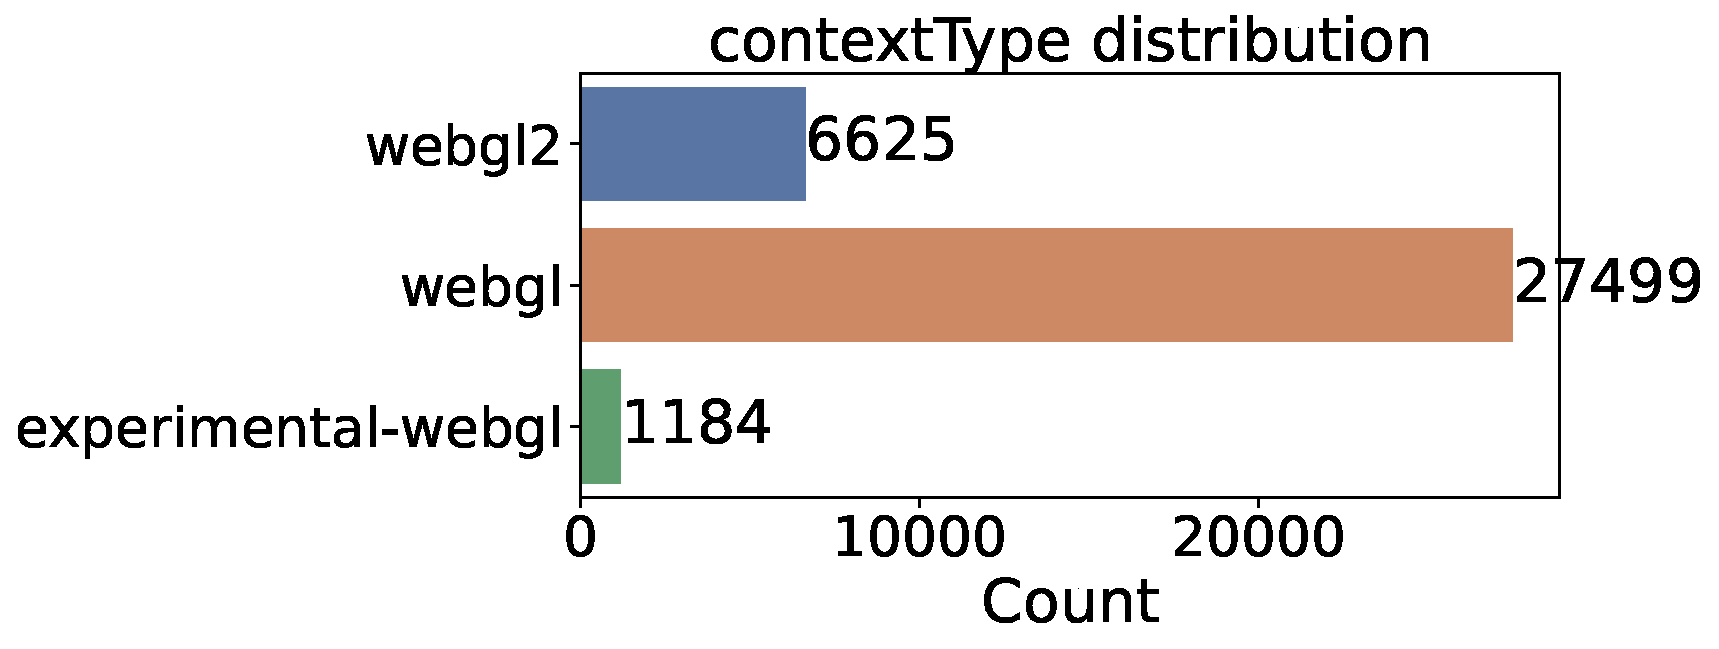
\includegraphics[width=0.4\textwidth]{figures/results_raf_contextType.pdf}
\caption{The Popularity of Context Type}\label{fig_context_type}
\end{figure}

We first examine the context attributes, which allow configuring various settings related to the WebGL context, such as alpha, depth, stencil, antialiasing, and power preference.

\subsubsection{Usage of WebGL Extensions.}

\begin{figure}[tp]
\centering
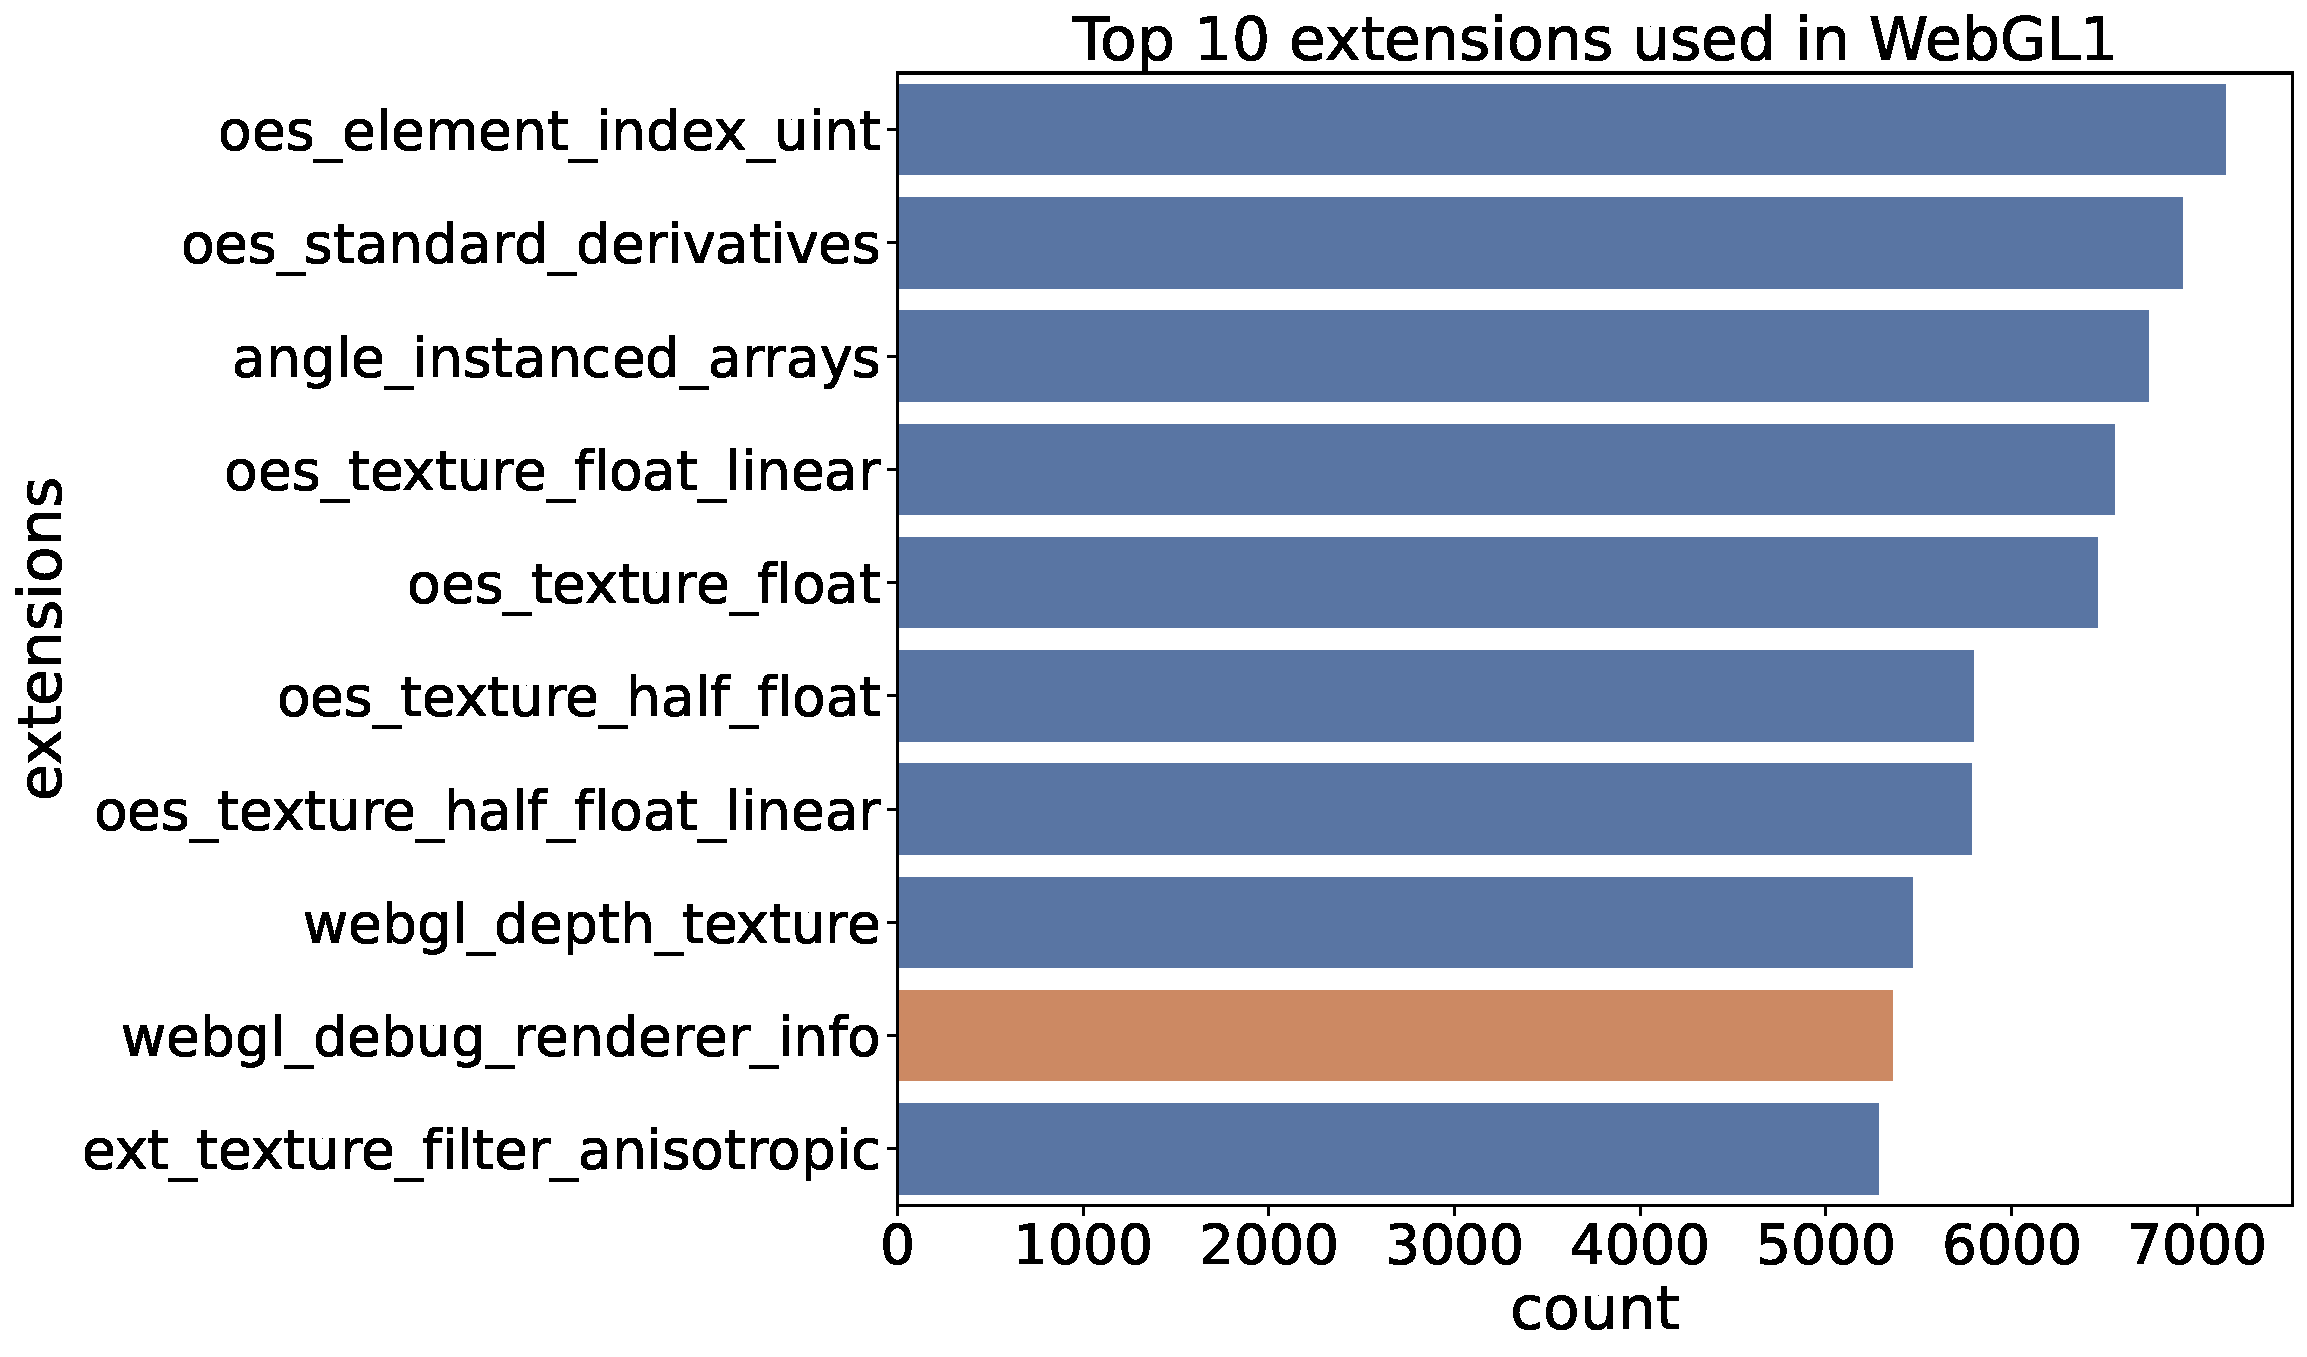
\includegraphics[width=0.4\textwidth]{figures/results_context_extensions.pdf}
\caption{Top 10 Popular WebGL Extensions}\label{fig_context_ext}
\end{figure}

\begin{figure}[tp]
\centering
\includegraphics[width=0.4\textwidth]{figures/results_temp_ext.png}
\caption{TEMP TEMP TEMP}\label{fig_temp_ext}
\end{figure}

WebGL extensions enhance the rendering capabilities of the WebGL API, providing developers with more options and flexibility for creating visually rich and high-performance web applications. However, not all extensions are supported by all devices. For instance, the \texttt{WEBGL\_compressed\_texture\_s3tc} extension is not supported by mobile web browsers.

We discovered that among the 34,256 contexts investigated, 21,664 contexts utilized WebGL extensions, accounting for 63.24\%.

Figure\ \ref{fig_context_ext} illustrates the popularity of the top 10 WebGL extensions most frequently employed by contexts. The vertical axis enumerates the shader names, while the horizontal axis denotes the number of contexts in which each shader appears, thereby representing its popularity. Among these, six extensions control texture sampling, two manage vertex attributes, one extension offers partial derivative computation operators for shaders, and another extension, \texttt{WEBGL\_debug\_renderer\_info}, has captured our interest. This extension exposes two constants containing information about the graphics driver for debugging purposes. Although this extension is employed by 6,118 contexts, 5,245 of these contexts have not compiled any shaders. Furthermore, among these 5,245 contexts, 4,782 contexts have six or fewer gl function calls.

We observe that real-world WebGL applications may employ some extensions that lack functional or control equivalents in WebGPU\@. Table \ref{fig_temp_ext} shows these extensions and the frequency of their appearance in contexts. For instance, the \texttt{OVR\_multiview2} extension was introduced to expedite the rendering of left and right viewpoints in WebXR\@. In WebXR scenarios, the render passes for the left and right eyes are likely to be identical, except for the camera matrix. Sequentially rendering two different pipelines for the same set of render passes would introduce additional overhead. OpenXR designers recognized this issue and introduced the \texttt{OVR\_multiview2} extension to accelerate this process. However, in WebGPU, we have not identified a functionally equivalent feature, even though support for multiview exists in Vulkan, one of WebGPU's backends.

We also find that while the total number of WebGL1 contexts using extensions is lower than the total number of WebGL2 contexts using extensions, the number of extensions used by WebGL1 contexts is greater than the number used by WebGL2 contexts.

% \begin{itemize}
%     \item \texttt{OES\_texture\_float\_linear} and \texttt{OES\_texture\_half\_float\_linear}: This extension enables linear filtering (interpolation) of floating-point or half-floating-point textures, which improves the visual quality of floating-point textures by smoothing transitions between texels. In WebGPU, linear filtering for floating-point textures is supported directly in the API, without requiring separate extensions.
%     \item \texttt{EXT\_texture\_filter\_anisotropic}: This extension provides support for anisotropic filtering, a technique that enhances texture quality when viewing surfaces at oblique angles. It helps reduce blurring and maintains crisp details in textures. Anisotropic filtering is supported as a native feature in WebGPU\@. Developers can enable it through the sampler settings.
%     \item \texttt{OES\_element\_index\_uint}: This extension allows the use of unsigned 32-bit integer indices for element index buffers, enabling the use of larger vertex arrays and improving the efficiency of rendering complex 3D models. WebGPU supports unsigned 32-bit integer indices for element index buffers natively, enabling more efficient rendering of complex 3D models.
%     \item \texttt{ANGLE\_instanced\_arrays}: This extension enables instanced rendering, allowing multiple instances of the same geometry to be drawn with a single draw call. It improves performance when rendering a large number of identical objects. WebGPU has built-in support for instanced rendering, allowing developers to draw multiple instances of the same geometry with a single draw call without requiring an extension.
%     \item \texttt{OES\_standard\_derivatives}: This extension provides support for the GLSL built-in functions dFdx, dFdy, and fwidth, which allow shader authors to compute the rate of change of quantities across screen space. These functions are useful for implementing various effects, such as procedural texturing, bump mapping, and antialiasing. Derivative functions like dFdx, dFdy, and fwidth are supported natively in WebGPU's shading language, WGSL\@.
%     \item \texttt{OES\_texture\_float} and \texttt{OES\_texture\_half\_float}: This extension enables the use of 32-bit floating-point or 16-bit half-floating-point textures, allowing for higher precision and dynamic range in texture data compared to traditional 8-bit or 16-bit textures. WebGPU supports floating-point textures with various precisions natively, including 16-bit half-floating-point and 32-bit full-floating-point textures.
%     \item \texttt{WEBGL\_debug\_renderer\_info}: This extension provides additional debugging information about the WebGL implementation, including the renderer and vendor strings. This information can be helpful for developers to identify implementation-specific behaviors or optimize their applications for specific hardware. WebGPU has a more consistent and well-defined behavior across different platforms, reducing the need for implementation-specific debugging information. However, it is possible that future debugging tools and extensions will be developed for WebGPU to provide even more detailed information.
%     \item \texttt{WEBGL\_depth\_texture}: This extension enables the use of depth textures, allowing for more efficient and accurate depth-based effects such as shadow mapping and depth-of-field. WebGPU natively supports depth textures, enabling efficient and accurate depth-based effects like shadow mapping and depth-of-field.
% \end{itemize}

\subsubsection{Usage of OffscreenCanvas.}

\begin{figure}[tp]
\centering
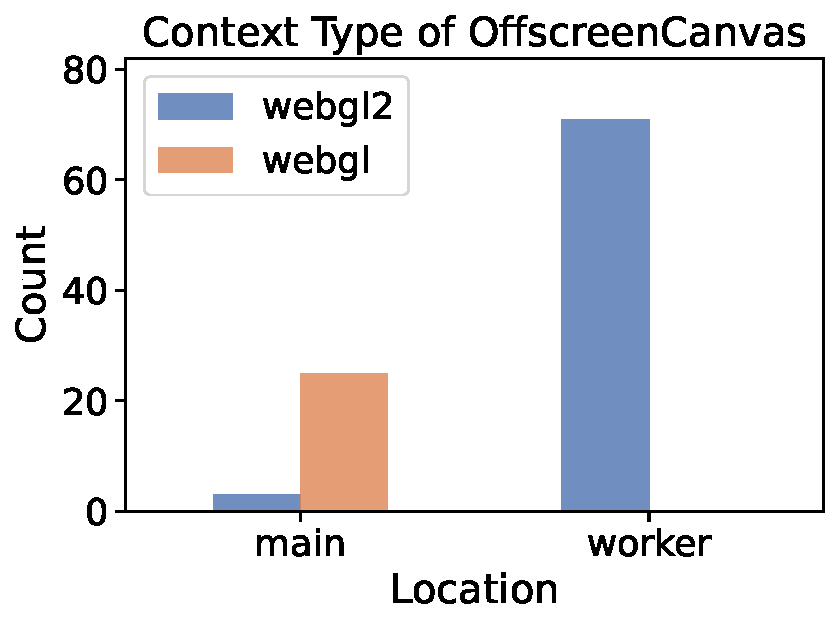
\includegraphics[width=0.4\textwidth]{figures/results_oc_type.pdf}
\caption{The usage of OffscreenCanvas}\label{fig_oc_type}
\end{figure}

\subsection{Duplicity of Pipelines}

% \hyd{Why the complexity and the duplicity(diversity) of WebGL shaders and pipelines are essential and important for our measurement study? Any potential benefit in the age of WebGPU?}

We measure the diversity of the rendering pipeline. Since WebGL applications assemble a global state to specify the rendering pipeline, evaluating the duplicity of the rendering pipeline can be equated to evaluating the duplicity of the global state. The possible value space for the WebGL pipeline in a single WebGL application is huge, since each WebGL function may change the global state. However, it is worth noting that we only need to concern ourselves with the pipeline at the time of draw commands, because at this point the CPU freezes the entire pipeline and then controls the GPU to render. Thus, we serialize the global state of the WebGL runtime upon the invocation of any drawing command. 
% Contemporary WebGL frameworks may employ a minimal edit distance construction approach when developing the pipeline, which entails making the fewest possible modifications to the global state for the subsequent draw. As a result, 
The global state on calling a draw command may suffer some redundancy, as it retains aspects of the previous draw command’s global state, such as unused textures or uniform buffers. Consequently, the duplicity analyzed in this section serves as a lower bound, with the actual duplicity potentially being higher.

\begin{figure}[tp]
\centering
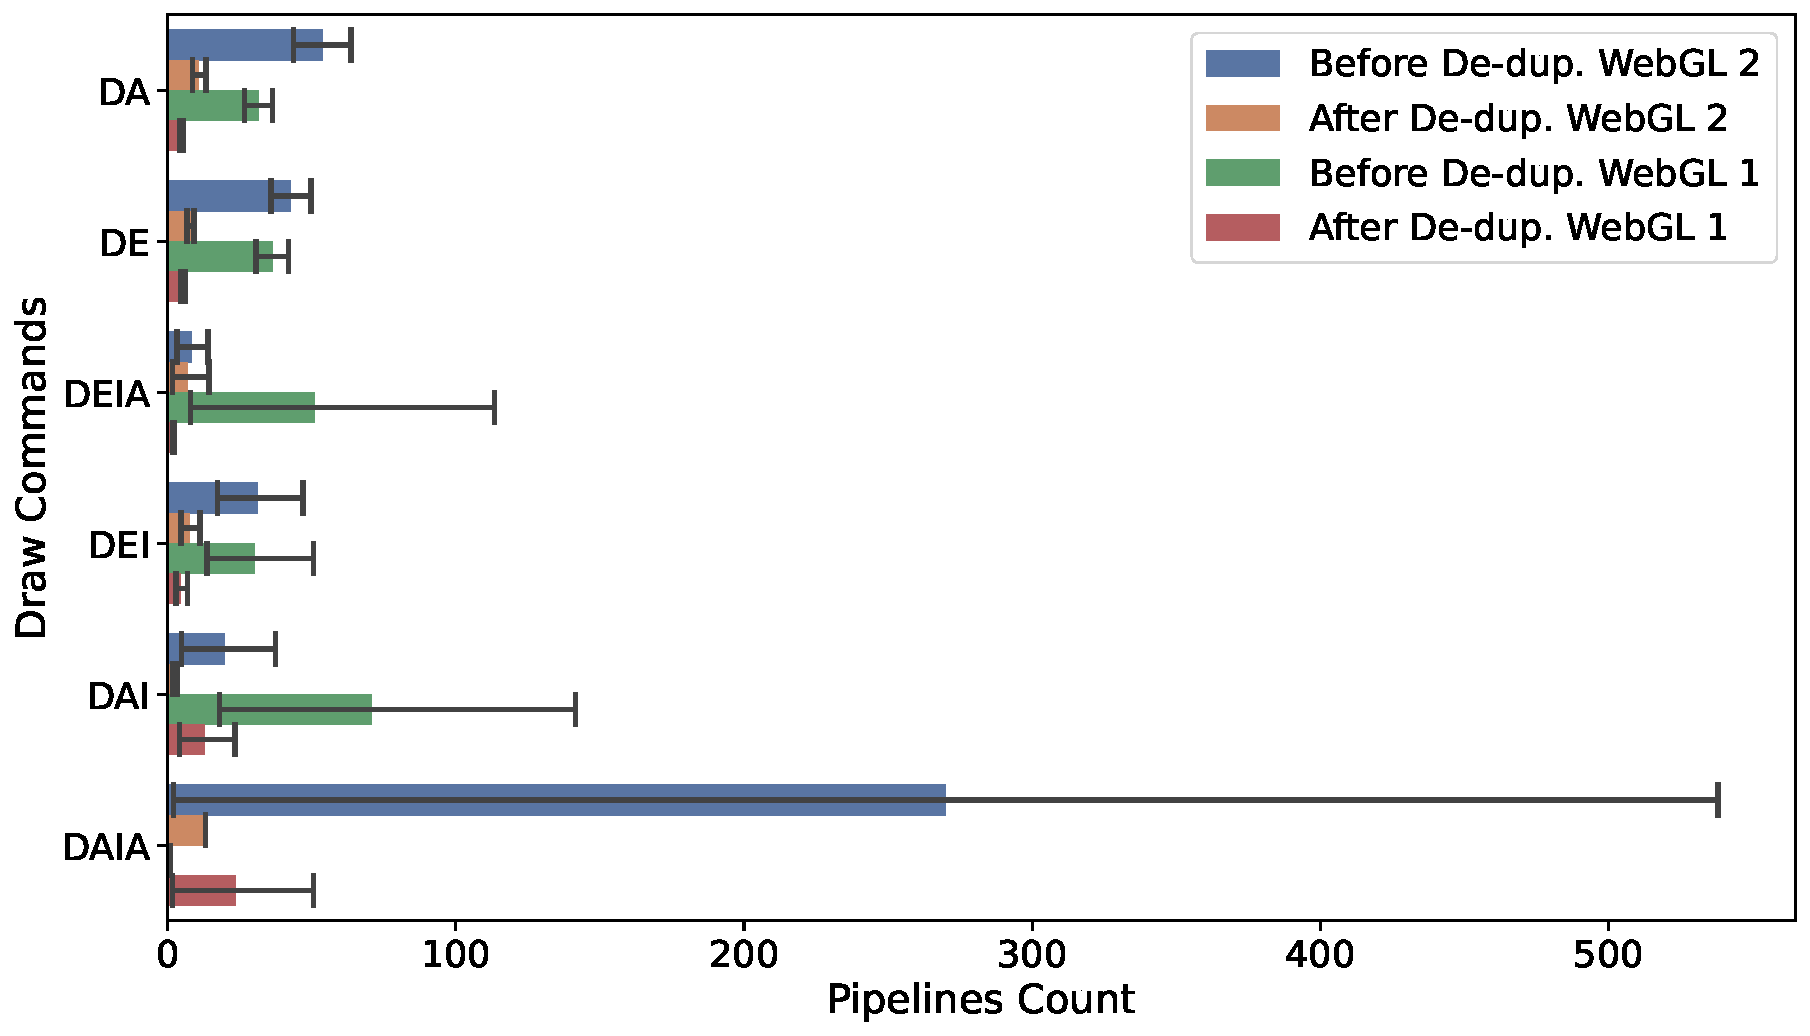
\includegraphics[width=0.95\linewidth]{figures/results_pipeline_dup.pdf}
\caption{Pipeline Duplicity of each Draw Commands}\label{fig_results_pipeline_dup}
\end{figure}

Figure\ \ref{fig_results_pipeline_dup} displays the distribution of pipeline duplicity within individual web pages across various WebGL websites. It is evident that in 90\% of these sites, the number of essentially distinct pipelines does not exceed 100. This observation implies the following:

There is potential for implementing pipeline caching mechanisms, such as designing a Pipeline Object (PO) analogous to the Vertex Array Object (VAO) or introducing corresponding pipeline caching in the browser.
% Upon transitioning to WebGPU, a maximum of 100 pipelines would be sufficient to render the most complex scenes.
% In the absence of data dependencies, for WebGL programs with multiple pipelines, leveraging WebGPU’s ability to assemble pipelines in multithreaded environments could yield up to a 100-fold performance improvement in pipeline assembly.

Regarding duplicity across websites, our primary focus is on the state control logic aspect of the pipeline. As uniform buffers and textures cannot be shared between different WebGL contexts, the significance of examining the entire pipeline’s duplicity between various websites is limited.

\subsection{Complexity to Assemble a Pipeline}

Developers invoke WebGL functions to assemble the pipeline. Functions that modify the global state between draw commands are associated with pipeline assembly. The assembled pipeline consists of a) control logic for the GPU program, such as the behavior in color state, stencil state, and depth test state, and b) resources attached to the pipeline. Therefore, measuring the complexity of the pipeline should incorporate the number of function calls, the lines of code for pipeline switching (assembling new pipelines), and the amount and types of resources.

\begin{figure}[tp]
\centering
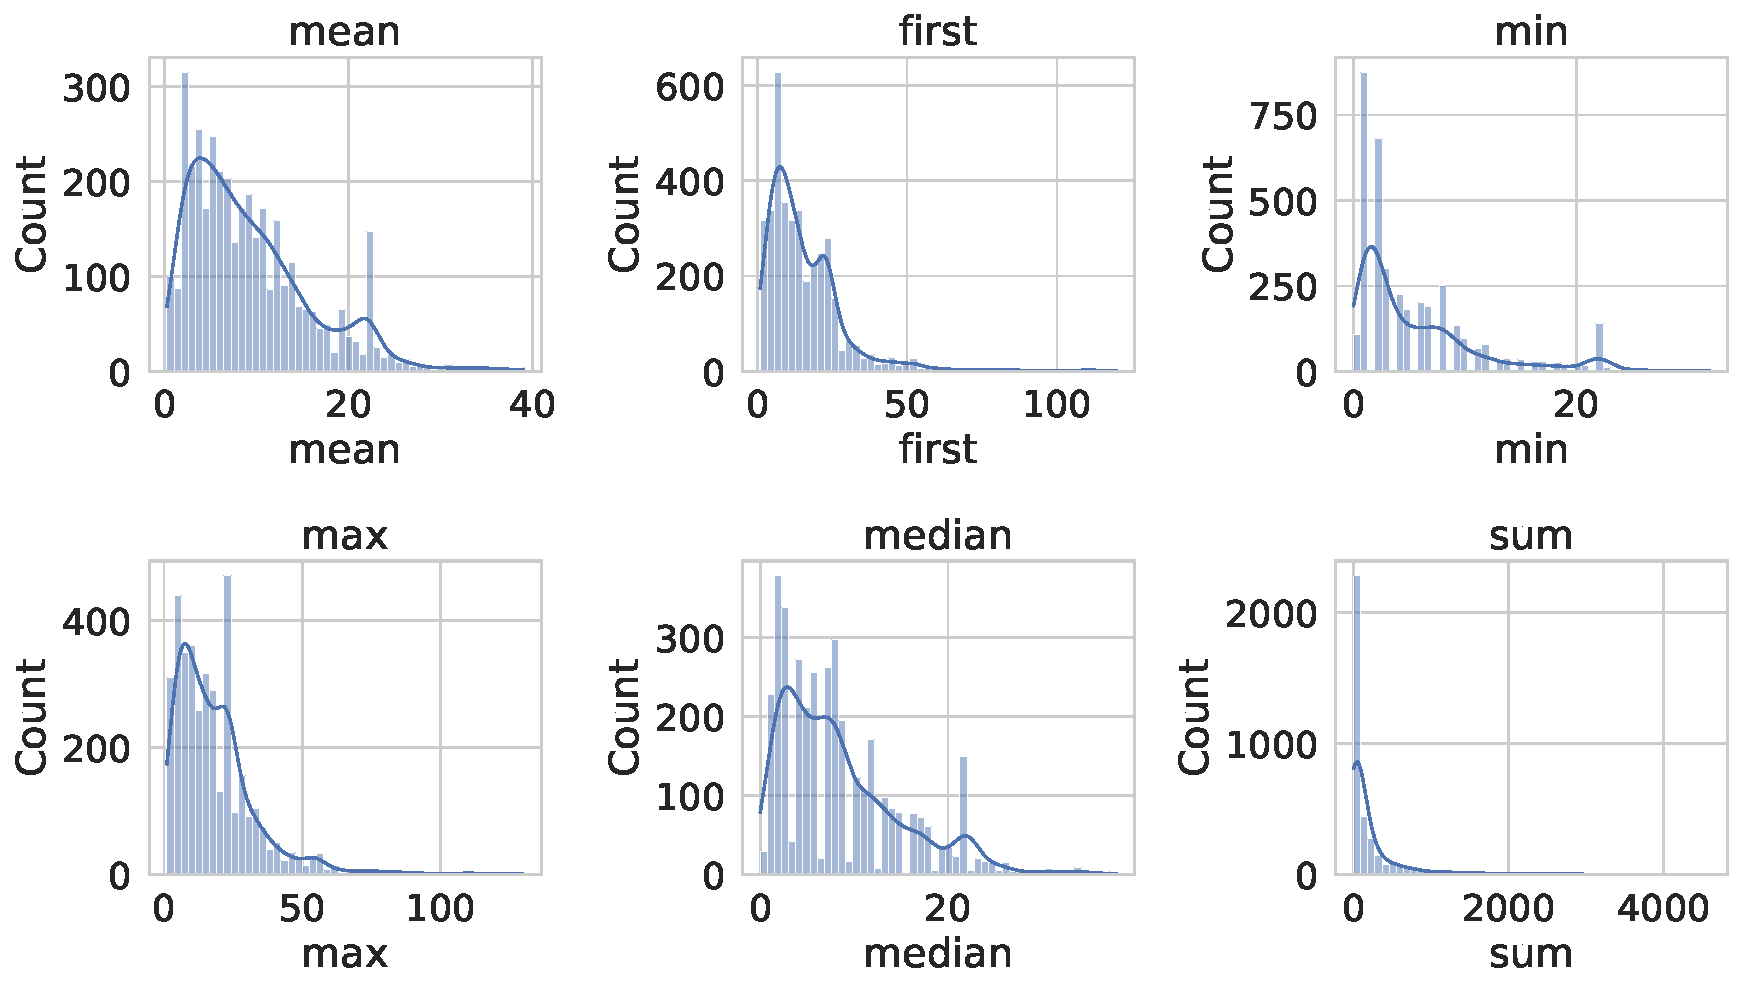
\includegraphics[width=0.95\linewidth]{figures/results_spector.pdf}
\caption{WebGL Invocations to Assemble a Pipeline}\label{fig_results_spector}
\end{figure}

\begin{figure}[tp]
\centering
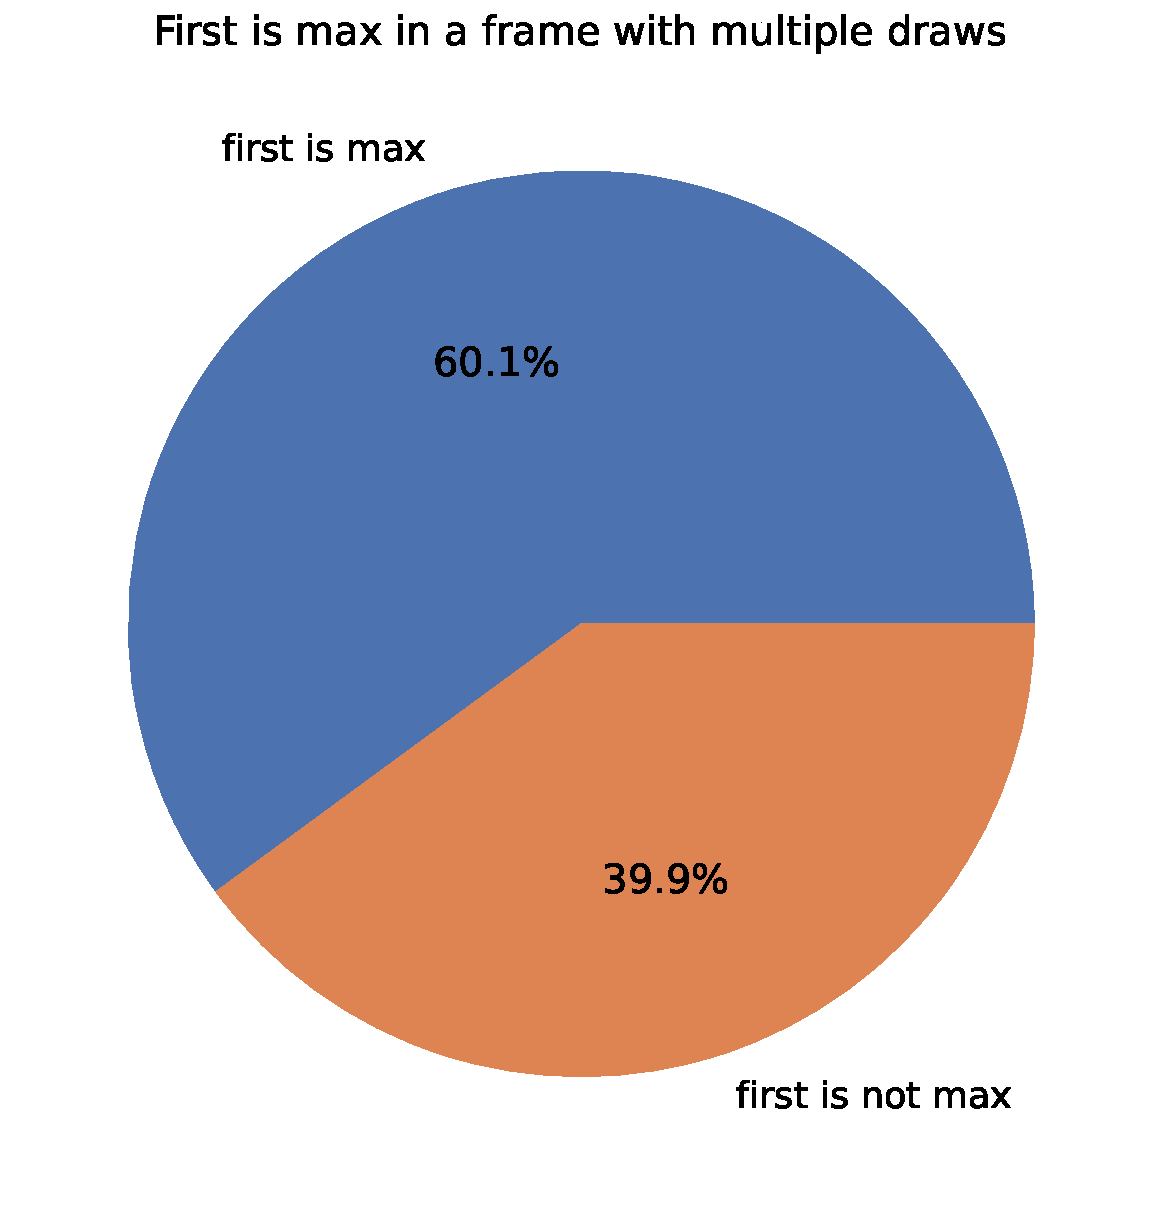
\includegraphics[width=0.95\linewidth]{figures/results_spector_first_is_max_in_multiple_draw.pdf}
\caption{First is Max in frame with multiple drawing commands}\label{fig_results_spector_first_is_max_in_multiple_draw}
\end{figure}


% \textbf{Number of calls.} % (raf)

% function calls
% triangles drawed.

\subsection{Usage of the Resources.} % (simple)


% resources(simple), number of function calls(raf), assembling complexity(spector-one) (几行语句装配管线?)

\subsection{Shaders}

% Since the shader instructs GPU what to do, the complexity of the shader is critical for user experience. Generally speaking, a complex shader indicates a fancy scene.
% Therefore we first examine the complexity of the shader. Then we study the duplicity of the shader. We conduct our measurement on 18,000 shaders gathered from 8000 different URLs. 

% https://developer.android.com/agi/frame-trace/shader-performance#shader_code_analysis

% \hyd{Why the complexity and the duplicity(diversity) of WebGL shaders and pipelines are \textbf{important} for our measurement study? Any potential benefit in the age of WebGPU?}

\subsubsection{Complexity.} Initially, we evaluate the complexity of the shaders by conducting a static analysis, as opposed to a dynamic analysis, which proves challenging for a isolated shader due to it is bound to render pipelines. In order to quantitatively measure these shaders, we examine various metrics, including shader length, abstract syntax tree (AST) depth, and the total number of nodes within the AST. Additionally, we investigate the utilization of global variables to further understand the shaders' complexity. Lastly, we also study the usage of transform feedback.

\textbf{Quantitative metric.}

\textbf{Global Variables.} 

\textbf{Transform feedbacks.}

% length, AST depth&nodes, Global Variables, transform feedbacks

\subsubsection{Duplicity.} A shader is duplicated if and only if its source code is the same as another shader's source code, regardless of the name of the variables. We conduct the shader's duplicity measurement by a GLSL parser. The results are shown in Fig X. The overall duplicity of the shaders is 77.29\%. Meanwhile, finding out the duplicity of the shaders across different websites is 67.96\%.


\begin{figure}[tp]
\centering
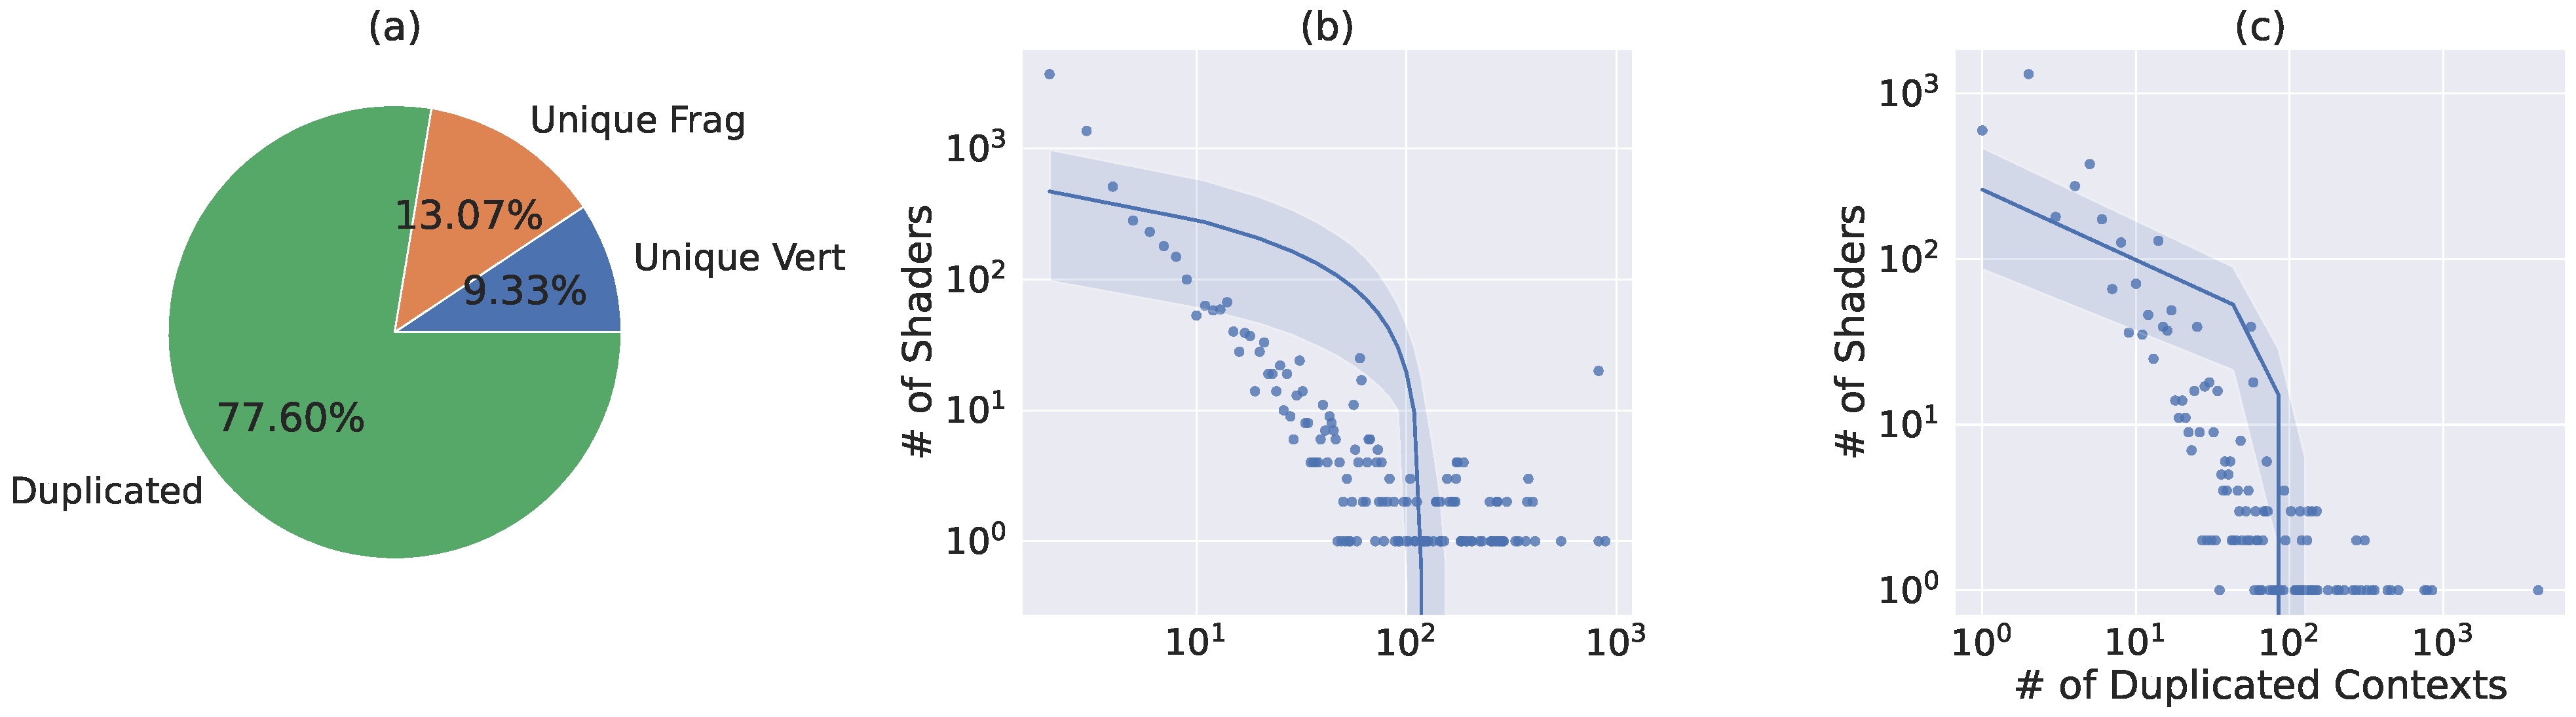
\includegraphics[width=0.4\textwidth]{figures/results_shader_duplicity.pdf}
\caption{The Duplicity of the Shaders}\label{fig_shader_dup}
\end{figure}

We find that the fragment shaders are more likely to be duplicated.

Fig X shows the top 50 popular shaders. The most popular shader is a fragment shader, which is used in 875 websites. However, we find it has a wired source code.

% precision mediump float;
% void main(void){
% float test = 0.1;
% if(test == 0.0){}
% else if(test == 1.0){}
% else if(test == 2.0){}
% else if(test == 3.0){}
% else if(test == 4.0){}
% else if(test == 5.0){}
% else if(test == 6.0){}
% else if(test == 7.0){}
% else if(test == 8.0){}
% else if(test == 9.0){}
% else if(test == 10.0){}
% else if(test == 11.0){}
% else if(test == 12.0){}
% else if(test == 13.0){}
% else if(test == 14.0){}
% else 
% gl_FragColor = vec4(0.0);
% }

We furthur analyze the relationship between the shader's length and the duplicity.

% \subsubsection{Transform Feedbacks.}

% For experiments on mobile phones, we used a Xiaomi Mi 6 phone with an 8-core processor and 6 GB memory, running Android OS. We collected the execution time and memory usage on mobile browsers using Android Debug Bridge (adb) [4]. The parameters we used with Google Chrome in each subsection of the evaluation are described in Appendix A.

\section{Related Work}

% Use case
    % TFJS
    % Threejs
    % Tracking(fingerprint)
% 3D graphics library: a survey 近年来,3D图形已经成为多媒体网络体验中越来越重要的一部分。继X3D标准的出现以及在网络上呈现3D图形的声明性方法的定义之后,WebGL的兴起使得低级别的图形硬件的访问能力不断增强。同时,远程渲染技术允许将高质量的3D图形流传到各种设备上,近年来还对基于网络的3D应用的内容传输方法进行了大量研究。所有这些发展都反映在3D网络越来越多的应用领域中。在本文中,我们通过对该领域的技术现状进行首次调查来反映这一活动。我们回顾了在浏览器中产生实时3D图形渲染的每一种主要方法,简要总结了3D图形远程渲染的方法,然后调查了数据压缩方法的补充研究,以及显著的应用领域。最后,我们评估了3D网络的影响和普及程度,回顾了过去并展望了未来。

Evan et.al.\ \cite{evans_3d_2014}

\section{Conclusion}

\section{Threat to Validity}
